\documentclass[12pt]{article}
\usepackage{amsmath}
\usepackage{physics}
\usepackage{amssymb}
\usepackage{graphicx}
\title{Homework 3}
\author{Patryk Kozlowski}
\date{\today}
\begin{document}
\maketitle


\section{Understanding the simple harmonic oscillator intuitively in a spatial basis}

\subsection{How we got \(a\) and \(a^{\dagger}\)}
This was done when we attempted to complete the square in our Hamiltonian, which went like $X^{2}+P^{2}$. We neglect the constant terms here. Thus, we got that our Hamiltonian factors to something like $(X+iP)(X-iP)$. We associated $a$ with $X+iP$ and $a^{\dagger}$ with $X-iP$.
\subsection{Define \(X\) and \(P\) in terms of \(a\) and \(a^{\dagger}\)}

We define \(X\) and \(P\), keeping track of the constants now, as follows:
\begin{equation}
    X = \sqrt{\frac{\hbar}{2m\omega}}(a^{\dagger} + a)
\end{equation}
\begin{equation}
    P = i\sqrt{\frac{m\omega\hbar}{2}}(a - a^{\dagger})
\end{equation}
\subsection{Calculation of \(\ev{X^2} \) and \(\ev{P^2}\)}

We define the expectation value of an operator as:
\begin{equation}
    \ev{A} = \bra{\Psi}A\ket{\Psi}
\end{equation}
Working in terms of the states of the simple harmonic oscillator, we first calculate \(\langle X^2\rangle\):
\begin{equation}
    \ev{X^2} = \bra{n}X^2\ket{n}
\end{equation}
Substituting in our expression for \(X\) from (1):
\begin{equation}
    = \frac{\hbar}{2m\omega}\bra{n}(a + a^{\dagger})^2\ket{n}
\end{equation}
Expanding the square:
\begin{equation}
    = \frac{\hbar}{2m\omega}\bra{n}(a^2 + a^{\dagger}a + aa^{\dagger} + (a^{\dagger})^2)\ket{n}
\end{equation}
The first and the last term will vanish due to orthonormality, so we just have to consider the middle terms:
\begin{equation}
    = \frac{\hbar}{2m\omega}\bra{n}(a^{\dagger}a + aa^{\dagger})\ket{n}
\end{equation}
Now, using our definitions for the action of \(a\) and \(a^{\dagger}\) on the states of the simple harmonic oscillator:
\begin{equation}
    a\ket{n} = \sqrt{n}\ket{n-1}
\end{equation}
\begin{equation}
    a^{\dagger}\ket{n} = \sqrt{n+1}\ket{n+1}
\end{equation}
First we consider the first term of equation 7:
\begin{equation}
\bra{n}a^{\dagger}a\ket{n} = \bra{n}a^{\dagger}\sqrt{n}\ket{n-1} = \sqrt{n}\sqrt{n}\bra{n}\ket{n}=n\bra{n}\ket{n}=n
\end{equation}
Now we consider the second term of equation 7:
\begin{equation}
\bra{n}aa^{\dagger}\ket{n} = \bra{n}\sqrt{n+1}\ket{n+1} = \sqrt{n+1}\sqrt{n+1}\bra{n}\ket{n}=(n+1)\bra{n}\ket{n}=n+1
\end{equation}
Now we can substitute these results back into equation 7:
\begin{equation}
   \ev{X^2} = \frac{\hbar}{2m\omega}(n + n + 1)\boxed{= \frac{\hbar}{2m\omega}(2n + 1)}
\end{equation}
Now we move on to the calculation of \(\ev{P^2}\):
\begin{equation}
    \ev{P^2} = \bra{n}P^2\ket{n}
\end{equation}
Since
\begin{equation}
    P = i\sqrt{\frac{m\omega\hbar}{2}}(a - a^{\dagger})
\end{equation}
\begin{equation}
    \ev{P^2} = -\frac{m\omega\hbar}{2}\bra{n}(a - a^{\dagger})^2\ket{n}
\end{equation}
Expanding the square:
\begin{equation}
    = -\frac{m\omega\hbar}{2}\bra{n}(a^2 - a^{\dagger}a - aa^{\dagger} + (a^{\dagger})^2)\ket{n}
\end{equation}
The first and the last term will vanish due to orthonormality, so we just have to consider the middle terms:
\begin{equation}
    = -\frac{m\omega\hbar}{2}\bra{n}(-a^{\dagger}a - aa^{\dagger})\ket{n}
\end{equation}
Now, using our definitions for the action of \(a\) and \(a^{\dagger}\) on the states of the simple harmonic oscillator:
\begin{equation}
    a\ket{n} = \sqrt{n}\ket{n-1}
\end{equation}
\begin{equation}
    a^{\dagger}\ket{n} = \sqrt{n+1}\ket{n+1}
\end{equation}
First we consider the first term of equation 17:
\begin{equation}
\bra{n}a^{\dagger}a\ket{n} = n
\end{equation}
Now we consider the second term of equation 17:
\begin{equation}
\bra{n}aa^{\dagger}\ket{n} = n+1
\end{equation}
Now we can substitute these results back into equation 17:
\begin{equation}
    = +\frac{m\omega\hbar}{2}(n + n + 1)\boxed{= \frac{m\omega\hbar}{2}(2n + 1)}
\end{equation}

\subsection{Uncertainty of Operators}

We start by calculating \(\Delta X\):
\begin{equation}
    \Delta X = \sqrt{\ev{X^2} - \ev{X}^2}
\end{equation}
We already have \(\ev{X^2}\) from part 3, so we just need to calculate \(\ev{X}\):
\begin{equation}
    \ev{X} = \bra{n}X\ket{n}
\end{equation}
Substituting in our expression for \(X\):
\begin{equation}
    = \sqrt{\frac{\hbar}{2m\omega}}\bra{n}(a + a^{\dagger})\ket{n}
\end{equation}
Due to the orthonormality of the states, both terms will vanish to give:
\begin{equation}
    \ev{X} = 0 \rightarrow \ev{X}^2 = 0
\end{equation}
So we have that:
\begin{equation}
    \Delta X = \sqrt{(\frac{\hbar}{2m\omega})(2n + 1)} =\boxed{\left(\frac{\hbar}{2m\omega}\right)^{\frac{1}{2}}\sqrt{2n + 1}}
\end{equation}
Next, we consider \(\Delta P\):
\begin{equation}
    \Delta P = \sqrt{\ev{P^2} - \ev{P}^2}
\end{equation}
We will have a similar argument why the second term vanishes, so we can just plug in our answer for the first term to get:
\begin{equation}
    \Delta P = \sqrt{(\frac{m\omega\hbar}{2})^{\frac{1}{1}}(2n + 1)} =\boxed{\left(\frac{m\omega\hbar}{2}\right)^{\frac{1}{2}}\sqrt{2n + 1}}
\end{equation}
So, we get the desired result of
\begin{equation}
    \boxed{\Delta X \Delta P = \frac{1}{2}(2n + 1)\hbar}
\end{equation}
\\
\subsubsection{Question}
Intuitively, what does this let us say about any wavefunction that satisfies the SHO solution to the perturbation of a potential minimum?

\textit{Hint:} Does the wavefunction become more or less spread in \(X\), \ldots
\subsubsection{Answer}
In the ground state of the oscillator with $n=0$, the uncertainty is at a minimum of $\frac{\hbar}{2}$. As $n$ increases, This total uncertainty will increase. So, as we move up in the rungs of the oscillator (which is a model system for any perturbation to a potential minimum), the minimum uncertainty increases i.e. the with function becomes more spread out in $X$ and $P$.
\section{Quantizing the Simple Harmonic Oscillator}

\textit{Objective:} To explore if quantizing the simple harmonic oscillator actually changes the kinetics, and if commutators of operators can really predict the time dependence of physical variables.

\subsection{Time Dependent State}
\subsubsection{Question}
A time dependent state satisfies $i\hbar \frac{d}{dt} |\Psi(t)\rangle = H|\Psi(t)\rangle$. Let $\Omega$ be any time-independent operator. Show that 
\[
\frac{d}{dt} \langle \Psi(t)|\Omega|\Psi(t)\rangle = \frac{i}{\hbar} \langle \Psi(t)|[H, \Omega]|\Psi(t)\rangle.
\]
\subsubsection{Solution}
We start by distributing the time derivative into all three elements of the left side of the equation:
\begin{equation}
    \frac{d}{dt} \langle \Psi(t)|\Omega|\Psi(t)\rangle =  \bra{\Psi(t)}\Omega\ket{\frac{d}{dt}\Psi(t)} + \bra{\Psi(t)}\frac{d}{dt}\Omega \ket{\Psi(t) } + \bra{\frac{d}{dt}\Psi(t)}\Omega\ket{\Psi(t)}
\end{equation}
We recognize:
\begin{equation}
    \frac{d}{dt}\ket{\Psi (t)} = \frac{1}{i\hbar}H\ket{\Psi (t)}
\end{equation}
Furthermore, we recognize that the adjoint of this is:
\begin{equation}
    \frac{d}{dt}\bra{\Psi (t)} = -\frac{1}{i\hbar}\bra{\Psi (t)}H
\end{equation}
Substituting these into equation 30:
\begin{equation}
    \frac{d}{dt} \langle \Psi(t)|\Omega|\Psi(t)\rangle =  \bra{\Psi(t)}\Omega\left(\frac{1}{i\hbar}H\ket{\Psi (t)}\right) + \bra{\Psi(t)}\frac{d}{dt}\Omega \ket{\Psi(t) } - \left(\frac{1}{i\hbar}\bra{\Psi (t)}H\right) \Omega\ket{\Psi(t)}
\end{equation}
We can confidently conclude that the middle term vanishes because \(\Omega\) is time independent e.g. $\frac{d}{dt}\Omega =0$. Pulling out the constance from the first and last terms, we get:
\begin{equation}
    \frac{d}{dt} \langle \Psi(t)|\Omega|\Psi(t)\rangle =  \frac{1}{i\hbar}\bra{\Psi(t)}\Omega H\ket{\Psi (t)} - \frac{1}{i\hbar}\bra{\Psi (t)}H\Omega\ket{\Psi(t)}
\end{equation}
We recognize the commutator:
\begin{equation}
    \frac{d}{dt} \langle \Psi(t)|\Omega|\Psi(t)\rangle =  \frac{1}{i\hbar}\bra{\Psi(t)}\Omega H\ket{\Psi (t)} - \frac{1}{i\hbar}\bra{\Psi (t)}H\Omega\ket{\Psi(t)} = \boxed{\frac{i}{\hbar}\bra{\Psi(t)}[H, \Omega]\ket{\Psi(t)}}
\end{equation}
\subsection{Harmonic Oscillator Specialization}
\subsubsection{Question}
Now specialize using part 1 to the harmonic oscillator. You will need to use the fact that
\[
\frac{i}{\hbar} [H, X] = \frac{1}{m} P \quad , \quad \frac{i}{\hbar} [H, P] = -m\omega^2X.
\]
For the harmonic oscillator, show that the expectation value of the position satisfies the classical equation of motion
\[
\left[ \frac{d^2}{dt^2} + \omega^2 \right] \langle \Psi(t)|X|\Psi(t)\rangle = 0.
\]
\subsubsection{Solution}
Since both the position and momentum operators are time independent we can substitute them for \(\Omega\) in the result from part 1. Starting from the left most term, we can make a substitution:
\begin{equation}
    \frac{d}{dt}\left(\frac{d}{dt}\bra{\Psi (t)}X\ket{\Psi (t)}\right) = \frac{d}{dt}\left(\bra{\Psi(t)}\frac{i}{\hbar}[H, X]\ket{\Psi(t)}\right)
\end{equation}
Now we can substitute in the commutator from the problem statement:
\begin{equation}
    \frac{d}{dt}\left(\bra{\Psi(t)}\frac{i}{\hbar}[H, X]\ket{\Psi(t)}\right) = \frac{d}{dt}\left(\bra{\Psi(t)}\left(\frac{1}{m}P\right)\ket{\Psi(t)}\right) = \frac{1}{m} \frac{d}{dt}\left(\bra{\Psi(t)}P\ket{\Psi(t)}\right)
\end{equation}
Now we can substitute in the result from part 1:
\begin{equation}
    = \frac{1}{m} \frac{i}{\hbar}\bra{\Psi(t)}[H, P]\ket{\Psi(t)} = \frac{1}{m} \bra{\Psi(t)}(-m\omega^{2}X)\ket{\Psi(t)} = -\omega^{2}\bra{\Psi(t)}X\ket{\Psi(t)}
\end{equation}
So, we have:
\begin{equation}
    \boxed{[  \frac{d^{2}}{dt^2} + \omega^2 ] \langle \Psi(t)|X|\Psi(t)\rangle = [ -\omega ^{2}+\omega ^{2} ] \langle \Psi(t)|X|\Psi(t)\rangle = 0}
\end{equation}
\subsection{Time Derivation and Operator Commutation}
\subsubsection{Question}
Show that for the harmonic oscillator
\[
\frac{d}{dt} \langle \Psi(t)|X^2|\Psi(t)\rangle = \frac{1}{m} \langle \Psi(t)|PX + XP|\Psi(t)\rangle.
\]
You will need $[H, AB] = [H, A]B + A[H, B]$.
\subsubsection{Solution}
Since the position squared is a time independent operator, we can use the relation from part 1:
\begin{equation}
    \frac{d}{dt} \langle \Psi(t)|X^2|\Psi(t)\rangle = \frac{i}{\hbar} \langle \Psi(t)|[H, X^2]|\Psi(t)\rangle
\end{equation}
Now, from the problem statement, we have that:
\begin{equation}
    [H, X^2] = [H, X]X + X[H, X] = \frac{\hbar}{im}\left(P X + XP\right)
\end{equation}
So, we can get our desired result:
\begin{equation}
    \frac{d}{dt} \langle \Psi(t)|X^2|\Psi(t)\rangle = \frac{i}{\hbar} \langle \Psi(t)| \frac{\hbar}{im}\left(P X + XP\right) |\Psi(t)\rangle = \boxed{\frac{1}{m} \langle \Psi(t)|PX + XP|\Psi(t)\rangle}
\end{equation}
\subsubsection{Question}
Then take another time derivative to show that
\[
\left[ \frac{d^2}{dt^2} + 4\omega^2 \right]\langle \Psi(t)|X^2|\Psi(t)\rangle = \frac{4}{m} \langle \Psi(t)|H|\Psi(t)\rangle.
\]
\subsubsection{Solution}
Will start by taking another time derivative of our previous result:
\begin{equation}
    \frac{d}{dt} \left(\frac{d}{dt} \langle \Psi(t)|X^2|\Psi(t)\rangle\right) = \frac{1}{m} \left(\frac{d}{dt}\langle \Psi(t)|PX|\Psi(t)\rangle+ \frac{d}{dt}\langle \Psi(t)|XP|\Psi(t)\rangle\right)
\end{equation}
We will first focus on the first term on the right side of the equality:
\begin{equation}
    \frac{d}{dt}\langle \Psi(t)|PX|\Psi(t)\rangle 
\end{equation}
in part 1, we found that:
\begin{equation}
    \frac{d}{dt}\langle \Psi(t)|PX|\Psi(t)\rangle = \frac{i}{\hbar}\langle \Psi(t)|[H, PX]|\Psi(t)\rangle
\end{equation}
Now,
\begin{equation}
   \frac{i}{\hbar} [H, PX] = \frac{i}{\hbar} [H, P]X + \frac{i}{\hbar} P[H, X] = -m\omega X^{2} +\frac{1}{m}P^{2}
\end{equation}
Likewise, for the other order, we have:
\begin{equation}
    \frac{i}{\hbar} [H, XP] = \frac{i}{\hbar} [H, X]P + \frac{i}{\hbar} X[H, P] = -m\omega X^{2} +\frac{1}{m}P^{2}
\end{equation}
So, we have that 
\begin{equation}
    \frac{d}{dt}\left(\frac{d}{dt} \langle \Psi(t)|X^2|\Psi(t)\rangle\right) = \frac{2}{m} \left(\langle\Psi (t)|\frac{P^{2}}{m}-m\omega X^{2}|\Psi (t)\rangle\right)= -2\omega ^{2} \langle\Psi (t)|X^{2}|\Psi (t)\rangle + \frac{2}{m^{2}} \langle\Psi (t)|P^{2}|\Psi (t)\rangle
\end{equation}
So we have cotton that:
\begin{equation}
    \left[ \frac{d^2}{dt^2} + 4\omega^2 \right]\langle \Psi(t)|X^2|\Psi(t)\rangle = \frac{2}{m^{2}} \langle\Psi (t)|P^{2}|\Psi (t)\rangle + 2\omega ^{2} \langle\Psi (t)|X^{2}|\Psi (t)\rangle
\end{equation}
Now we consider that:
\begin{equation}
    H = \frac{P^{2}}{2m} + \frac{1}{2}m\omega ^{2}X^{2} 
\rightarrow \frac{4}{m}H = \frac{2}{m^{2}}P^{2} + 2\omega ^{2}X^{2}
\end{equation}
This matches what we got above, so:
\begin{equation}
    \boxed{\left[ \frac{d^2}{dt^2} + 4\omega^2 \right]\langle \Psi(t)|X^2|\Psi(t)\rangle = \frac{2}{m^{2}} \langle\Psi (t)|P^{2}|\Psi (t)\rangle + 2\omega ^{2} \langle\Psi (t)|X^{2}|\Psi (t)\rangle = \frac{4}{m} \langle \Psi(t)|H|\Psi(t)\rangle}
    \end{equation}

\subsection{Classical Harmonic Oscillator}
\subsubsection{Question}
The solution to the classical harmonic oscillator is $x_{Cl} = x_0 \cos(\omega t + \phi)$ and the energy is $E_{Cl} = \frac{1}{2} m\omega^2 x_0^2$. Show that 
\[
\left[ \frac{d^2}{dt^2} + 4\omega^2 \right] x_{Cl}^2 = \frac{4}{m} E_{Cl}.
\]
\subsubsection{Solution}
We square the solution to the classical harmonic isolator:
\begin{equation}
    x_{Cl}^{2} = x_{0}^{2}\cos^{2}(\omega t + \phi)
\end{equation}
First, we take one derivative with respect to time, invoking they chain role. Treating $x_{0}^{2}$ as a constant, we get on to the nasty algebra
% go stop by stop in this deviation
\begin{equation}
    \frac{d}{dt}x_{Cl}^{2} = -x_{0}^{2}(2\cos(\omega t + \phi)(-\sin(\omega t + \phi)\omega)) = -\omega x_{0}^{2} \sin({2(\omega t + \phi)})
\end{equation}
Now we take another derivative with respect to time:
\begin{equation}
    \frac{d}{dt}\frac{d}{dt}x_{Cl}^{2} = -\omega x_{0}^{2}(2\cos(\omega t + \phi)\omega) = -2\omega^{2}x_{0}^{2}\cos(2(\omega t + \phi))
\end{equation}
Now, plugging in the equation from the problem statement:
\begin{equation}
    \left[ \frac{d^2}{dt^2} + 4\omega^2 \right] x_{Cl}^2 = -2\omega^{2}x_{0}^{2}\cos(2(\omega t + \phi)) + 4\omega^{2} \left(x_{0}^{2}\cos^{2}(\omega t + \phi)\right)
\end{equation}
Now, we have the relation
\begin{equation}
    \cos^{2}(x) = \frac{1}{2}(1 + \cos(2x))\rightarrow\cos^{2}(\omega t + \phi) = \frac{1}{2}(1 + \cos(2(\omega t + \phi)))
\end{equation}
So, we can substitute this in to get:
\begin{equation}
    \left[ \frac{d^2}{dt^2} + 4\omega^2 \right] x_{Cl}^2 = -2\omega^{2}x_{0}^{2}\cos(2(\omega t + \phi)) + 4\omega^{2} x_{0}^{2}\left(\frac{1}{2}(1 + \cos(2(\omega t + \phi)))\right)
\end{equation}
\begin{equation}
    = -2\omega^{2}x_{0}^{2}\cos(2(\omega t + \phi)) + 2\omega^{2} x_{0}^{2} + 2\omega^{2} x_{0}^{2}\cos(2(\omega t + \phi)) = 2\omega^{2} x_{0}^{2}
\end{equation}
Now, for the right and side we have
\begin{equation}
    \frac{4}{m} E_{Cl} = \frac{4}{m}\frac{1}{2} m\omega^{2}x_{0}^{2} = 2\omega^{2} x_{0}^{2}
\end{equation}
So, we have that:
\begin{equation}
    \boxed{\left[ \frac{d^2}{dt^2} + 4\omega^2 \right] x_{Cl}^2 = 2\omega^{2} x_{0}^{2} =  \frac{4}{m} E_{Cl}}
\end{equation}
\subsubsection{In other words, intuitively, does it make any change if we solve for our dynamics using only operator commutations?}
Know, it doesn't and the algebra is much simpler :)

\section{Problem 3}

For this problem, let’s explore raising and lowering operators in something that’s not quite a simple harmonic oscillator (SHO). The kinetic energy is the same as the SHO, but let’s define our potential as a quartic: 
\[ V(x) = \frac{k}{2}x^4 \]
We will assume that \( \omega = \sqrt{\frac{k}{m}} \) still holds.

\subsection{Write the Hamiltonian of this system. (Hint: think kinetic + potential)}
\begin{equation}
    H = \frac{p^2}{2m} + \frac{k}{2}x^4 = \frac{p^2}{2m} + \frac{1}{2}m \omega ^{2}x^{4}= \frac{1}{2m} \left(p^{2} + m^{2}\omega^{2}x^{4}\right)= \frac{1}{2m} \left(p^{2} + \left(m \omega x^{2}\right)^{2}\right)
\end{equation}
\subsection{`Factor' the Hamiltonian of the quartic potential into the product of two terms. Define the “+” factor as \( b \) and the “-” factor as \( b^\dagger \). (Hint: you should get something that looks like the SHO, but with \( x^2 \) instead of \( x \))}
In the privies section, we ot for the hambletonian:
\begin{equation}
    H = \frac{1}{2m} \left(p^{2} + \left(m \omega x^{2}\right)^{2}\right)
\end{equation}
Completing the square, defining $p=c$ and $m \omega x^{2}=d$, we get:
\begin{equation}
    H = \frac{1}{2m} \left(c^{2} + d^{2}\right) = \frac{1}{2m} \left(\left(c+id\right)\left(c-id\right)\right)
\end{equation}
Substituting in for c and d, we find
\begin{equation}
    H = \frac{1}{2m} \left(\left(p+im \omega x^{2}\right)\left(p-im \omega x^{2}\right)\right)
\end{equation}
Now we are in a place to define $b$ and $b^{\dagger}$:
\begin{equation}
    b = \sqrt{\frac{m\omega}{2\hbar}}x^2 + \frac{i}{\sqrt{2m\omega\hbar}}p
\end{equation}
\begin{equation}
    b^{\dagger} = \sqrt{\frac{m\omega}{2\hbar}}x^2 - \frac{i}{\sqrt{2m\omega\hbar}}p
\end{equation}
\subsection{What is \( b^\dagger b \)? (Hint: calculate the commutator of \( x^2 \) with \( \hat{p} \))}
We will first look at the first term:
\begin{equation}
    b^\dagger b = \left(\sqrt{\frac{m\omega}{2\hbar}}x^2 - \frac{i}{\sqrt{2m\omega\hbar}}p\right)\left(\sqrt{\frac{m\omega}{2\hbar}}x^2 + \frac{i}{\sqrt{2m\omega\hbar}}p\right)
\end{equation}
multiplying out, we get
\begin{equation}
    b^\dagger b = \frac{m\omega}{2\hbar}x^4 + \frac{1}{2m\omega\hbar}p^2 + \frac{i}{2\hbar}\left(x^{2}p- px^{2}\right) = \frac{m\omega}{2\hbar}x^4 + \frac{1}{2m\omega\hbar}p^2 + \frac{i}{2\hbar}\left([x^{2},p]\right)
\end{equation}
We can use the relation
\begin{equation}
    [x^{2},p] = x[x,p] + [x,p]x = x\left(i\hbar\right) + \left(i\hbar\right)x = 2i\hbar x
\end{equation}
So, we can substitute this in to get:
\begin{equation}
    b^\dagger b = \frac{m\omega}{2\hbar}x^4 + \frac{1}{2m\omega\hbar}p^2 + \frac{i}{2\hbar}\left(2i\hbar x\right) \boxed{= \frac{m\omega}{2\hbar}x^4 + \frac{1}{2m\omega\hbar}p^2 - x}
\end{equation}
\subsection{Rewrite the Hamiltonian of the quartic oscillator in terms of the product \( b^\dagger b \) that you calculated in the previous step. How is energy in a quartic oscillator different from an SHO?}
\begin{equation}
    H = \hbar \omega \left(\frac{m\omega}{2\hbar}x^4 + \frac{1}{2m\omega\hbar}p^2 -x+x \right)= \hbar \omega \left(b^{\dagger}b +x\right)
\end{equation}
In the SHO, we had:
\begin{equation}
    H = \hbar \omega \left(a^{\dagger}a +\frac{1}{2}\right)
\end{equation}
So, instead of the anergy depending on a constant term, it depends on the position of the particle.
We get an energy spacing is still separated by $\hbar \omega$, but depends an the position, as shown in this image:
\begin{figure}[h]
    \centering
    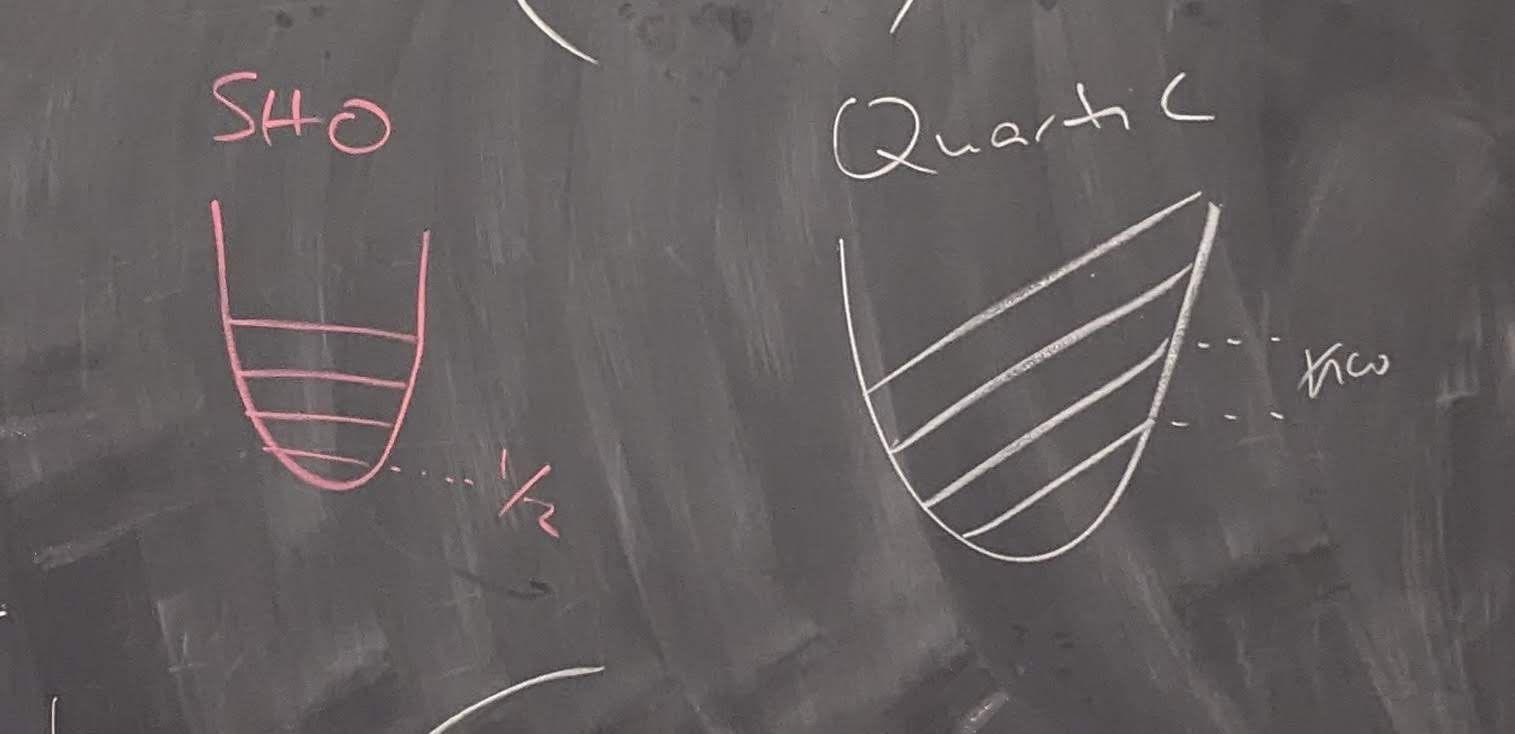
\includegraphics[width=0.5\textwidth]{quartic.png}
    \caption{Energy levels of the quartic oscillator}
    \label{fig:mesh1}
\end{figure}


\end{document}